\chapter{Методы обучения на данных со слабой разметкой} \label{chapt2}

\section{Обзор существующих методов} \label{sect2_1}

Обучение сегментации на слабо размеченных данных, особенно в случае, когда разметка относится к изображению целиком без каких-либо геометрических привязок(как примерное местоположение аномалий, размер. и т.п.) - такую слабую разметку будем называть {\bf низкоуровневой} - представляется по меньшей мере неочевидной задачей. При разработке системы, допускающей такое обучение, необходимо каким-то образом связать геометрию маски сегментации на всем множестве её пикселей, со значением разметки низкого уровня для данного изображения.

В работе \cite{lu_survey_2018} приводится обзор существующих методов решения данной задачи. Главным образом необходимо выделить следующие:

\begin{itemize}
    \item Обучение на множестве объектов (Multiple instance learning) - MIL - о нём пойдет речь ниже;
    \item Методы обучения, использующие и интегрирующие ограничения(к примеру, на количество пикселей положительного класса) в процесс обучения;
    \item Методы, связанные с автокодировщиками(\cite{alex_semisupervised_2017}) и generative adversarial network (GAN);
\end{itemize}


\noindent При этом подход MIL считается в большей степени классическим и традиционным, чем остальные, при обучении сегментации на данных со слабой разметкой. Данный подход будет описан подробнее в следующем параграфе.

\section{MIL}

Метод {\bf Multiple instance learning} является переходным между классической классификацией и классической сегментацией.
При обучении пиксели рассматриваются с одной стороны как элементы, определяющие классификацию всего изображения(наличие хоть одного
<<положительного>> пикселя влечёт присвоение всему изображению положительного класса, а отсутствие - отрицательного), а с другой - 
каждый пиксель <<ответственен>> за локализацию опухоли как в классической задаче сегментации. С тем чтобы добиться такой интерпретации, 
используется специальная функция потерь специального вида(\cite{zhu_deep_2016}). Сперва положим, что существует некоторая свёрточная нейронная сеть(с коэффициентами $\theta$) M, на вход которой подаются изображения $I_n$ и которая возвращает карту сегментации R. Карта может быть меньшей размерности(тогда нужно снизить размерность и разметки), чем иходное изображение. Занумеруем пиксели карты  от 1 до m и обозначим их $r_1, \dots, r_m$, занумеруем изображения $I_1, \dots, I_N$. Метка(низкоуровневая разметка данных) $y=1$ будет обозначать наличие на изображении пикселей положительного класса, а $y = 0,$  соответственно, отсутствие таковых. Пусть $(r_1', r_2',\dots, r_m') := sort(r_1, \dots, r_m )$ обозначает сортировку массива $r_1, \dots, r_m$ по убыванию. В свёрточных нейронных сетях значение $r_i'$ будет зависеть лишь от какой-то части $Q_i'$ изображения I. Зафиксируем параметр $K\in\mathbb{N}$ и обозначим: 
$$p(y=1|Q_i', \theta):= r_i', ~p(y=0|Q_i', \theta):= 1 - r_i'.$$ Тогда определим функцию потерь следующим образом:

\begin{equation}
  \label{eq:equation1}
  \mathcal{L} := -\frac{1}{mN}\sum_{n=1}^N\left( \sum_{j=1}^K\log(p(y_n|Q_{j}'^n,\theta)+\sum_{j=K+1}^m\log(p(y=0|Q_{j}'^n,\theta))\right)
\end{equation}


Для получения карты R используют различные техники.  С развитем техник глубинного обучения многие авторы при обработке изображений 
для получения карты R стали часто прибегать к использованию свёрточных нейронных сети(\cite{quellec_multiple-instance_2017}).

Существуют и иные разновидности MIL. Так, к примеру, вместо того, чтобы заранее предопределять долю <<положительных>> пикселей в карте R путём введения параметра K, можно добавить в функцию потерь регуляризационный член, отвечающий за контроль суммарной массы карты R. Тогда система <<сама>> будет определять, в каком количестве и куда этот вес распределять. Примером реализации такой идеи может служить функция потерь следующего вида: 


\begin{equation}
  \label{eq:equation2}
  \mathcal{L} := \frac{1}{N}\sum_{n=1}^N\left(-\log(p(y_n|I_n,\theta)) + \mu||r_n'||_1\right)
\end{equation}


\section{Эксперименты с MIL и комментарии к ним}


Эксперименты с MIL проводились с набором данных CBIS-DDSM(\cite{lee_curated_2017}), в котором представлены снимки более 6 тысяч пациентов, с диагностированным  злокачественным или доброкачественным новообразрванием молочных желёз. При подготовке эксперимента был учёт опыт \cite{zhu_deep_2016}, параметры обучения и данные INbreast, которые использовались наряду с данными CBIS-DDSM, были взяты в основном оттуда. О характере сходимости метода можно сказать следующее:

\begin{itemize}
    \item Метод чувствителен к значению параметра K;
    \item Метод чувствителен к размерности карты сегментации: на картах меньшей размерности сходимость метода к визуально интерпретируемым результатам наблюдалась стабильнее; при больших размерностях карты уместно сбалансировать весом  функцию потерь, чтоб количество единиц и нулей при подсчёте функции потерь \ref{eq:equation1} не отличалось в большое число раз;
    \item Метод чувствителен к значению параметра $\mu$ в \ref{eq:equation2}: слишком жёсткое ограничение на регуляризацию не позволяет достаточно свободно оптимизировать  первое слагаемое функции потерь;
    \item Эффективность метода также зависит от набора данных: на экспериментах с набором данных INbreast результаты были стабильнее;
\end{itemize}




\subsubsection{Архитектура}

Для экспериментов была выбрана нейросеть ResNet-50, имеющая близкие к оптимальным показатели на наборе данных ImageNet. Последний свёрточный слой данной сети возвращает пиксельную карту размером 7x7, которая и используется для реализации метода MIL($m = 49$)(рис. \ref{fig:schema_mil}). 


\begin{figure}[h] 
  \center
  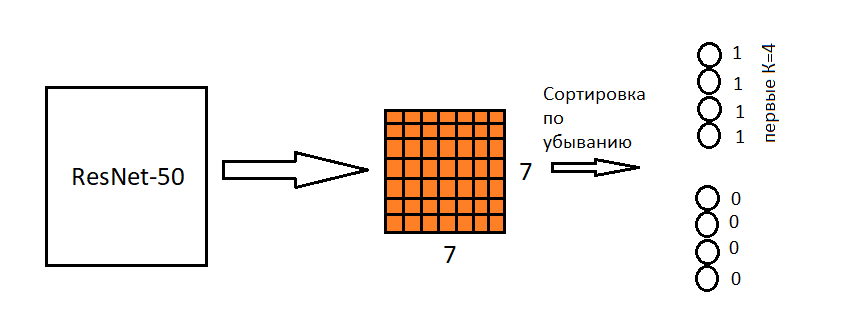
\includegraphics [scale=0.8] {images/schema_mil.png}
  \caption{Схема метода MIL} 
  \label{fig:example_mil}  
\end{figure}

\subsubsection{Примеры изображений и анализ результатов}


\begin{figure}[h] 
  \center
  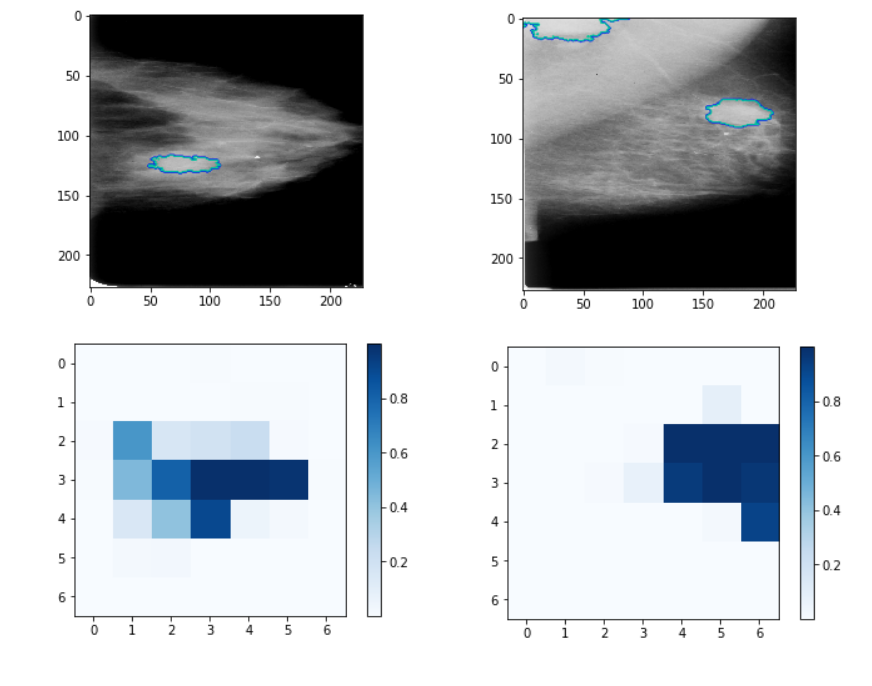
\includegraphics [scale=0.6] {images/mil.png}
  \caption{Примеры оригинальных изображений с контуром новообразования(верхний ряд) и карт сегментации к ним(нижний ряд), K = 4} 
  \label{fig:schema_mil}  
\end{figure}


На основе проделанных экспериментов были сделаны следующие выводы относительно особенностей метода MIL с точки зрения задачи сегментации:

\begin{itemize}
    \item Разрешение 7x7, где один пиксель зачастую покрывает контур новообразования целиком, не даёт четкого представления об этом контуре при сегментации;
    \item MIL требует значительной и довольно тонкой подстройки параметров, что усложняет его применимость;
    \item Алгоритм не всегда выделяет только то, что следует, а также часто выделяет ложно интерпретируемые артефакты(рис. \ref{fig:example_mil} - справа);
    \item Однако нельзя отрицать, что данный алгоритм действительно способен извлекать некоторую геометрическую информацию из слабой разметки;
    
\end{itemize}


На основе сделанных выводов было принято решение попытаться использовать MIL в виде инструмента подстройки сегментации, получаемой на сильно размеченном набора данных относительно {\bf небольшого} размера.

